% Compile with:  pdflatex worldstrat_aoi_report.tex  (twice, for the references)
% The tables, figures and \newcommand values are produced by ../analyze_aoi_bias.py
\documentclass[11pt,a4paper]{article}

\usepackage[T1]{fontenc}
\usepackage[utf8]{inputenc}
\usepackage[margin=2.4cm]{geometry}
\usepackage{booktabs}
\usepackage{graphicx}
\usepackage{amsmath}
\usepackage{xcolor}
\usepackage[font=small,labelfont=bf]{caption}
\usepackage{float}
\usepackage[hidelinks]{hyperref}

\graphicspath{{figures/}}
\newcommand{\NAOI}{3\,928}
\newcommand{\NLandcover}{2\,407}
\newcommand{\SettlementShare}{43}
\newcommand{\SettlementShareLC}{61}
\newcommand{\UrbanShare}{29}
\newcommand{\MedianNN}{39.6}
\newcommand{\ClusteredShare}{18}
\newcommand{\WithinFifty}{55}
\newcommand{\OverlapPairs}{7\,169}
\newcommand{\OverlapSites}{723}
\newcommand{\CrossSplitPairs}{2\,504}


\newcommand{\ratio}[1]{$\times#1$}
\setlength{\parskip}{0.4em}
\setlength{\parindent}{0pt}

\title{\vspace{-1.5cm}A Global Area-of-Interest List for the Sentinel-2 L1C Pipeline\\
\large Coordinates from WorldStrat and a Representativeness Analysis}
\author{Khalil Bibi}
\date{\today}

\begin{document}
\maketitle

\begin{abstract}
\noindent
This note delivers the input needed to launch a full dataset build with our Sentinel-2 L1C
pipeline: a list of \NAOI{} areas of interest (AOIs) taken from the WorldStrat dataset, a
builder that regenerates it from the official metadata, and a batch driver that feeds it to the
pipeline site by site. It then asks whether that list is a \emph{representative} sample of the
land surface. It is not, and the deviations are large and systematic: built-up areas are
over-represented by roughly two orders of magnitude (\SettlementShare\% of AOIs versus about
1\% of the ice-free land surface), temperate and tropical climates are over-represented
(\ratio{1.9} and \ratio{1.5}), polar and arid climates under-represented (\ratio{0.2} and
\ratio{0.8}), and Oceania and Antarctica are almost absent. The AOIs are also strongly
clustered: \ClusteredShare\% lie closer to another AOI than the width of one footprint, which
creates \OverlapPairs{} overlapping pairs, \CrossSplitPairs{} of them straddling two different
WorldStrat splits. None of this makes the list unusable, and for super-resolution it is a
deliberate and reasonable design, but any model trained on the resulting dataset will inherit
these priors. The report quantifies each bias against a land-area reference and lists concrete
mitigations.
\end{abstract}

\section{Purpose and deliverables}

The pipeline (\texttt{s2\_l1c\_pipeline.py}) turns a coordinate and a date range into a
pixel-aligned time series of $13\times1024\times1024$ \texttt{uint16} arrays at 10\,m
resolution. To move from single locations to a full dataset, three pieces are added to the
repository:

\begin{itemize}
  \item \texttt{sites/worldstrat\_aoi.csv} --- \NAOI{} AOI centres with their WorldStrat
        attributes (\texttt{site\_id}, \texttt{lat}, \texttt{lon}, \texttt{source},
        \texttt{ipcc\_class}, \texttt{lccs\_class}, \texttt{smod\_class}, \texttt{split});
  \item \texttt{build\_worldstrat\_aoi.py} --- regenerates that CSV from the official WorldStrat
        metadata on Zenodo (two files, $\approx$15\,MB; the imagery archives are not needed);
  \item \texttt{run\_sites.py} --- runs the pipeline over any CSV with \texttt{lat}/\texttt{lon}
        columns, one output folder per site, with throttling, retries, sharding and resume.
\end{itemize}

The analysis of Sections~\ref{sec:method}--\ref{sec:results} is reproduced by
\texttt{analyze\_aoi\_bias.py}, which writes every figure, table and number used here.

\section{The AOI list}

\subsection{Provenance}

WorldStrat \cite{worldstrat} samples the land surface for a super-resolution benchmark and
publishes its AOI metadata under CC-BY-4.0 (Zenodo record 6810792). Its AOIs come from four
sampling sources, which explains most of what follows:

\begin{center}
\begin{tabular}{lrl}
\toprule
Source & AOIs & Sampling rationale \\
\midrule
Landcover  & 2\,407 & stratified over land-cover classes \\
UNHCR      & 981    & refugee settlements \\
ASMSpotter & 351    & artisanal and small-scale mining sites \\
Amnesty    & 189    & human-rights points of interest \\
\bottomrule
\end{tabular}
\end{center}

Three of the four are \emph{purposive} samples of human activity. This is entirely appropriate
for the original goal --- the dataset was built to train super-resolution models on scenes that
matter to humanitarian work --- but it means the list was never meant to be an equal-area sample
of the planet, and it should not be used as one without correction.

\subsection{Footprint mismatch}
\label{sec:footprint}

A WorldStrat AOI covers $2.5\,\mathrm{km}^2$ (about $1.6\times1.6$\,km). Our footprint is
$10.24\times10.24$\,km, i.e.\ $104.9\,\mathrm{km}^2$, roughly $42\times$ larger. Each AOI centre
therefore yields a much wider scene than the original tile. Two consequences run through the
rest of this report: neighbouring AOIs that were disjoint in WorldStrat now overlap
(Section~\ref{sec:clustering}), and the land-cover label attached to an AOI describes only its
central $2.4\%$ --- the surrounding scene may be something else entirely.

\subsection{Running the list}

\begin{verbatim}
# 1. (re)build the list from the official metadata
python build_worldstrat_aoi.py

# 2. check what a subset would download, without downloading
python run_sites.py --sites sites/worldstrat_aoi.csv --output_root data/worldstrat \
    --limit 20 --start_date 2023-01-01 --end_date 2023-12-31 --max_cloud 20 --dry_run

# 3. real run: the 4 clearest scenes of 2023 per site, resumable
python run_sites.py --sites sites/worldstrat_aoi.csv --output_root data/worldstrat \
    --start_date 2023-01-01 --end_date 2023-12-31 --max_cloud 20 \
    --max_images 4 --sort cloud

# 4. shard across machines
python run_sites.py ... --skip 0    --limit 1000
python run_sites.py ... --skip 1000 --limit 1000
\end{verbatim}

Every option not consumed by the driver is forwarded to the pipeline unchanged, so per-site
behaviour (cloud limit, quality control, access mode) is exactly the single-site behaviour.
Progress is appended to \texttt{sites\_progress.csv}; re-running the same command skips
finished sites, and within a site the pipeline skips dates already on disk.

\section{Method}
\label{sec:method}

The question is whether the AOIs are distributed like the land surface. For each category $c$
(climate class, continent, latitude band) we compare the sample share $p_c$ with the share of
global land area $q_c$ and report the \emph{representation ratio}
\begin{equation}
  r_c = \frac{p_c}{q_c},
\end{equation}
so $r_c>1$ means over-representation. Land-area references come from two public datasets:

\begin{itemize}
  \item \textbf{Climate:} the Köppen--Geiger map of Beck et al.\ \cite{koppen}, 5~arcmin, used
        both to label each AOI and --- weighting every cell by $\cos\varphi$ --- to compute the
        share of global land in each climate class. It also defines the land mask used for the
        latitude reference.
  \item \textbf{Continents:} Natural Earth 1:110m country polygons, with geodesic areas on the
        WGS84 ellipsoid.
\end{itemize}

We test each distribution with a $\chi^2$ goodness-of-fit against the land-area expectation, and
summarise the size of the deviation with the total variation distance
$\mathrm{TVD}=\tfrac12\sum_c|p_c-q_c|$, i.e.\ the fraction of the sample that would have to be
relocated for the two distributions to match. Clustering is measured with great-circle distances
between AOI centres.

A caveat on the $\chi^2$ tests: with \NAOI{} AOIs, any deviation is statistically significant,
and the sample was never drawn at random, so the $p$-values confirm rather than discover. The
ratios and the TVD carry the useful information.

\section{Results}
\label{sec:results}

\subsection{Geographic coverage}

\begin{figure}[H]
\centering
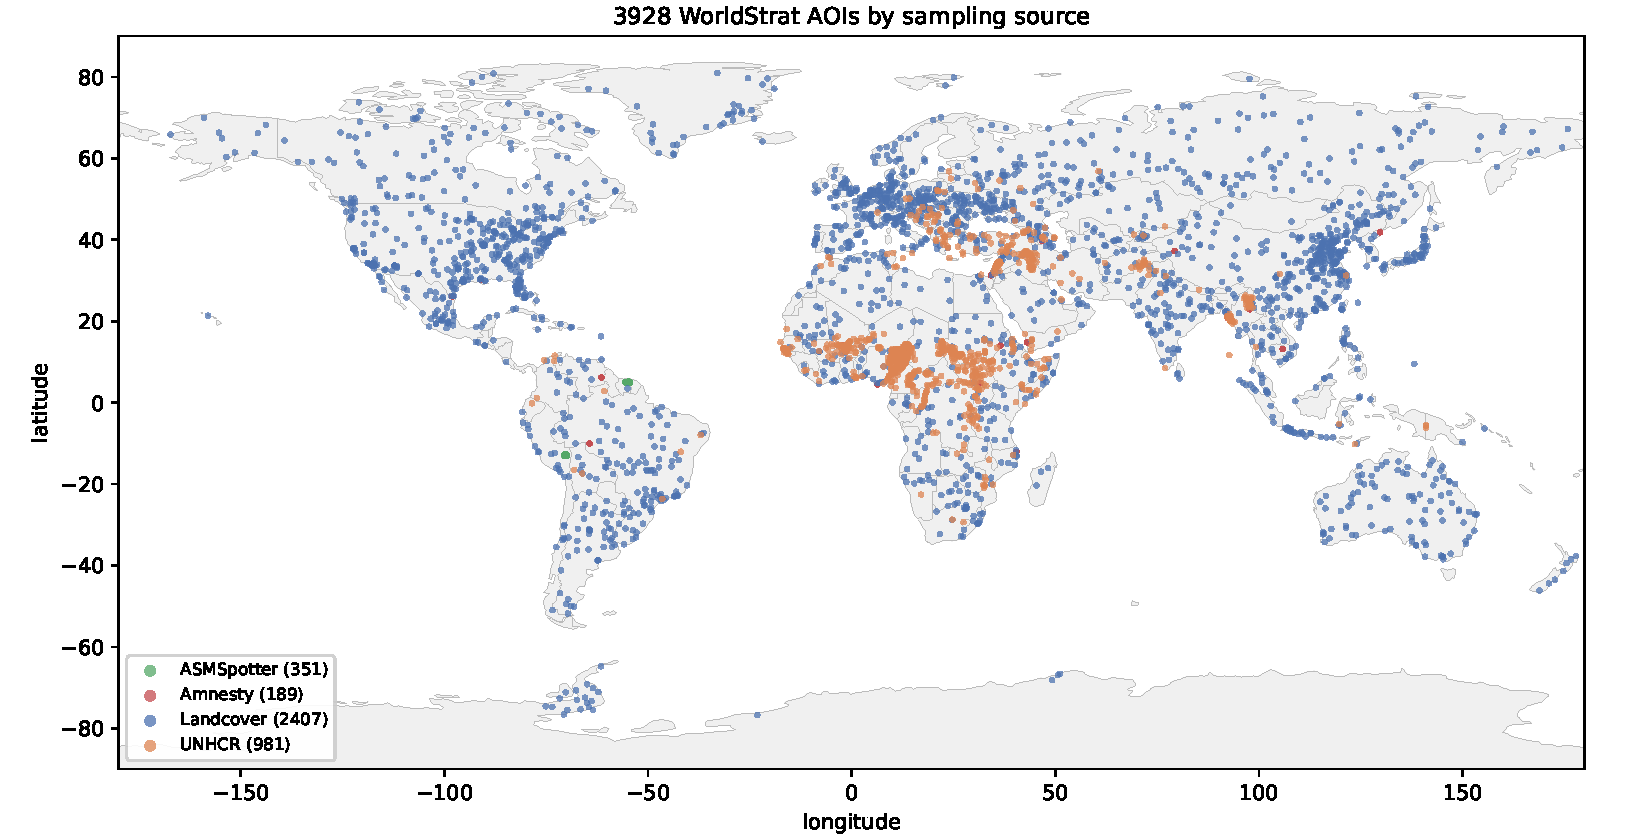
\includegraphics[width=\textwidth]{aoi_world_map.pdf}
\caption{The \NAOI{} AOIs, coloured by sampling source. The Landcover stratum spreads
worldwide, while the three thematic sources concentrate in the Sahel, the Middle East, South-East
Asia and the Guiana Shield.}
\label{fig:map}
\end{figure}

Continents deviate moderately from land area ($\mathrm{TVD}=0.14$, $\chi^2=503$, 6 d.o.f.,
$p<10^{-100}$). Africa is over-represented (\ratio{1.31}) and Asia, Europe and South America sit
close to parity, but Oceania (\ratio{0.45}) and especially Antarctica (\ratio{0.07}) are thin.
Antarctica is a defensible omission for most applications; Oceania is not.

\begin{table}[H]
\centering
\caption{AOIs per continent against share of global land area.}
\begin{tabular}{lrrrr}
\toprule
Continent & AOIs & sample (\%) & land (\%) & ratio \\
\midrule
Africa & 1042 & 26.5 & 20.3 & 1.31 \\
Asia & 985 & 25.1 & 21.2 & 1.18 \\
Europe & 665 & 16.9 & 15.7 & 1.08 \\
South America & 576 & 14.7 & 12.1 & 1.22 \\
North America & 535 & 13.6 & 16.6 & 0.82 \\
Oceania & 103 & 2.6 & 5.8 & 0.45 \\
Antarctica & 22 & 0.6 & 8.4 & 0.07 \\
\bottomrule
\end{tabular}

\label{tab:continents}
\end{table}

The latitude profile (Figure~\ref{fig:latitude}) shows the northern mid-latitudes
($30^\circ$--$60^\circ$N, 40.0\% of AOIs for 31.5\% of land) and the tropics over-weighted, while
everything above $60^\circ$N (\ratio{0.35}) and the southern high latitudes are sparse
($\mathrm{TVD}=0.20$).

\begin{figure}[H]
\centering
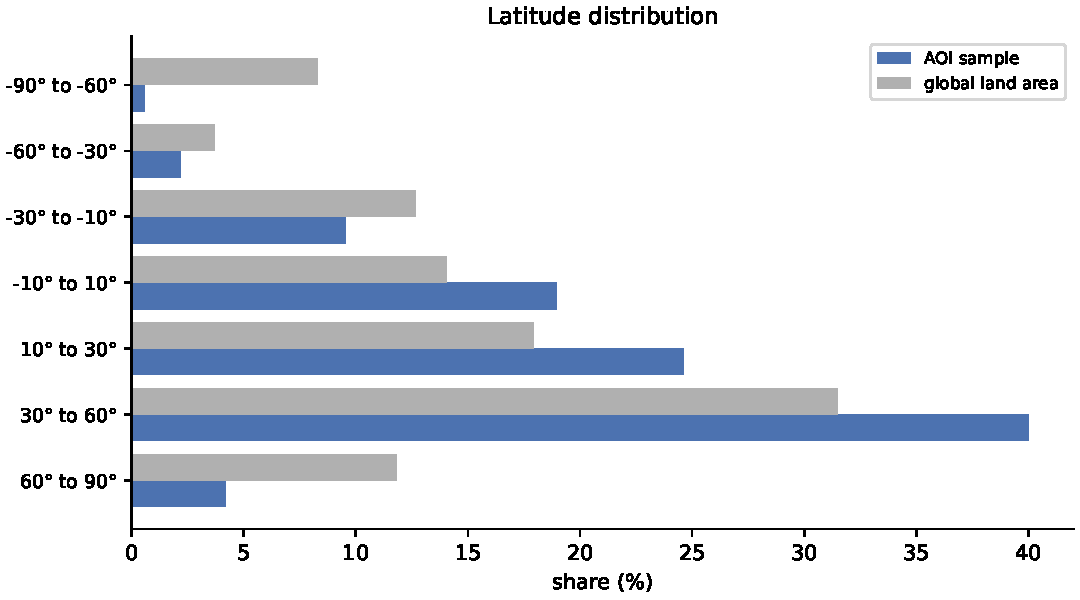
\includegraphics[width=0.78\textwidth]{latitude.pdf}
\caption{Latitude distribution of the AOIs against the distribution of land area.}
\label{fig:latitude}
\end{figure}

\subsection{Climate and biomes}

Climate is where the sample departs most from the land surface ($\mathrm{TVD}=0.21$:
about one AOI in five would have to move to a different climate to match land area).

\begin{table}[H]
\centering
\caption{Köppen--Geiger main groups. The ratio is the sample share divided by the land share.}
\begin{tabular}{lrrrr}
\toprule
Climate group & AOIs & sample (\%) & land (\%) & ratio \\
\midrule
Tropical & 1191 & 30.4 & 20.0 & 1.52 \\
Arid & 995 & 25.4 & 31.1 & 0.82 \\
Temperate & 855 & 21.8 & 11.2 & 1.94 \\
Cold & 762 & 19.4 & 22.6 & 0.86 \\
Polar & 121 & 3.1 & 15.1 & 0.20 \\
\bottomrule
\end{tabular}

\label{tab:koppen}
\end{table}

\begin{figure}[H]
\centering
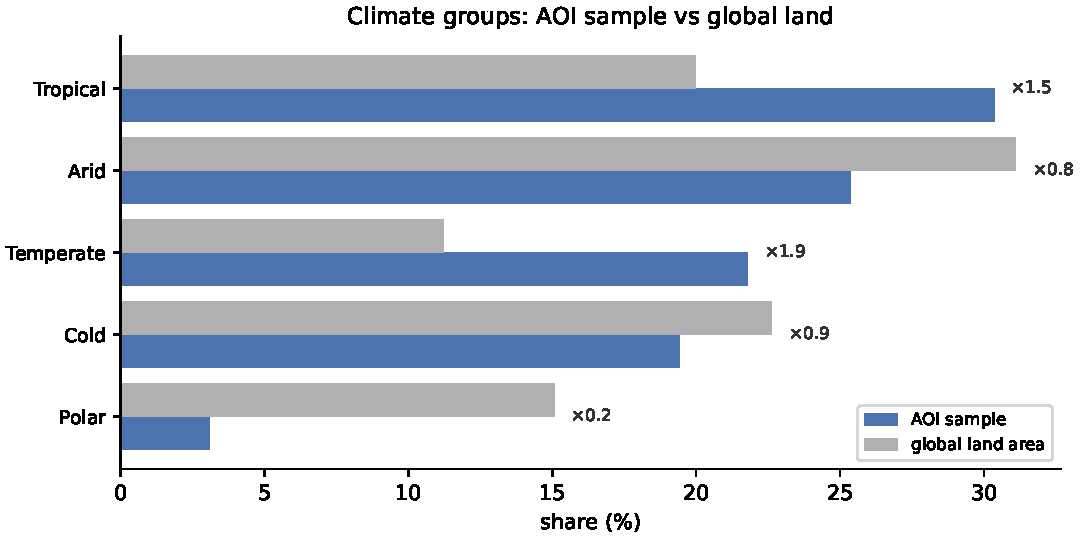
\includegraphics[width=0.85\textwidth]{koppen_groups.pdf}
\caption{Climate groups: sample versus global land area, with representation ratios.}
\label{fig:koppen}
\end{figure}

Two effects dominate. Temperate climates (group C, \ratio{1.94}) are over-sampled because
people, cities and the humanitarian points of interest that seeded three of the four sources are
concentrated there; tropical climates (group A, \ratio{1.52}) are lifted by the mining and
refugee sites. Conversely, polar and high-mountain climates (group E, \ratio{0.20}) and the
world's deserts and steppes (group B, \ratio{0.82}) are under-sampled --- together they are
46\% of the land surface but 28\% of the AOIs. At the level of individual classes
(Appendix~\ref{app:classes}), the gaps are sharper: the hot desert class BWh, 14.7\% of global
land, holds 9.1\% of AOIs (\ratio{0.62}), and the boreal Dfc class drops to \ratio{0.34}.

A model trained on this dataset will therefore see comparatively little snow, ice, sand and
boreal forest --- the surfaces whose radiometry is least like the temperate scenes it will see
most often.

\subsection{Land cover and built-up bias}

\begin{figure}[H]
\centering
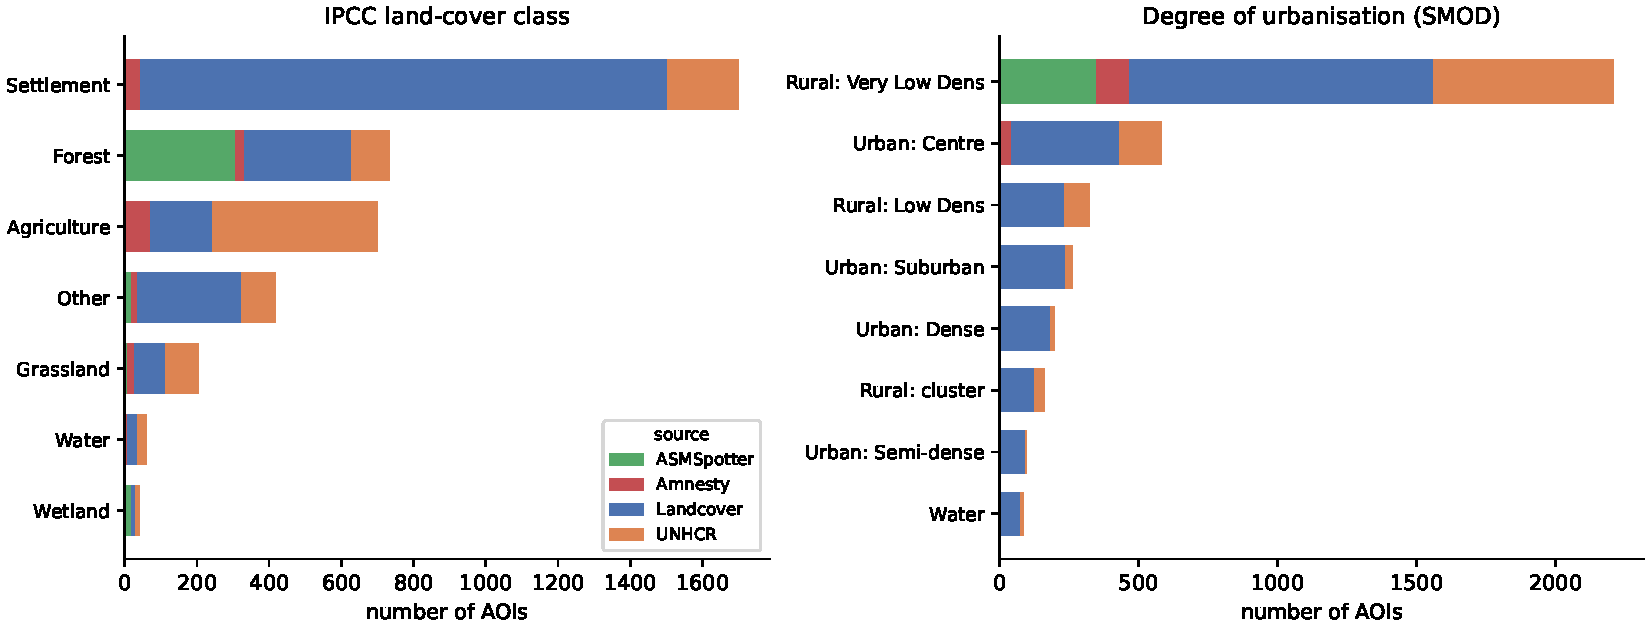
\includegraphics[width=\textwidth]{composition.pdf}
\caption{Land-cover class and degree of urbanisation, split by sampling source.}
\label{fig:composition}
\end{figure}

The strongest bias is land cover. \SettlementShare\% of the AOIs are labelled
\emph{Settlement} and \UrbanShare\% fall in an urban SMOD class, whereas built-up land covers on
the order of 1\% of the ice-free land surface \cite{ghsl}. That is an over-representation of
roughly two orders of magnitude --- far larger than any climatic or geographic effect measured
above.

It would be natural to blame the humanitarian sources, but the numbers say otherwise:
\SettlementShareLC\% of the \NLandcover{} AOIs in the Landcover stratum are also settlements.
Whatever stratification produced that subset, it was not proportional to land area either. The
practical consequence is that the built-up prior is structural and cannot be removed by dropping
the UNHCR, ASMSpotter and Amnesty sites.

Two secondary observations:
\begin{itemize}
  \item Water and wetland classes are marginal (59 and 41 AOIs), so coastal and inundated
        scenes are scarce.
  \item The labels describe the central $1.6\times1.6$\,km of a $10.24\times10.24$\,km scene
        (Section~\ref{sec:footprint}). A \emph{Settlement} AOI in our dataset is usually a town
        surrounded by whatever landscape contains it, which softens --- but does not remove ---
        the imbalance at the pixel level.
\end{itemize}

\subsection{Spatial clustering and split leakage}
\label{sec:clustering}

WorldStrat AOIs often come in tight groups (e.g.\ \texttt{ASMSpotter-1-1-1..3}). The median
distance from an AOI to its nearest neighbour is \MedianNN{}\,km, \ClusteredShare\% of AOIs are
closer to another AOI than one footprint width, and \WithinFifty\% have a neighbour within 50\,km.

\begin{figure}[H]
\centering
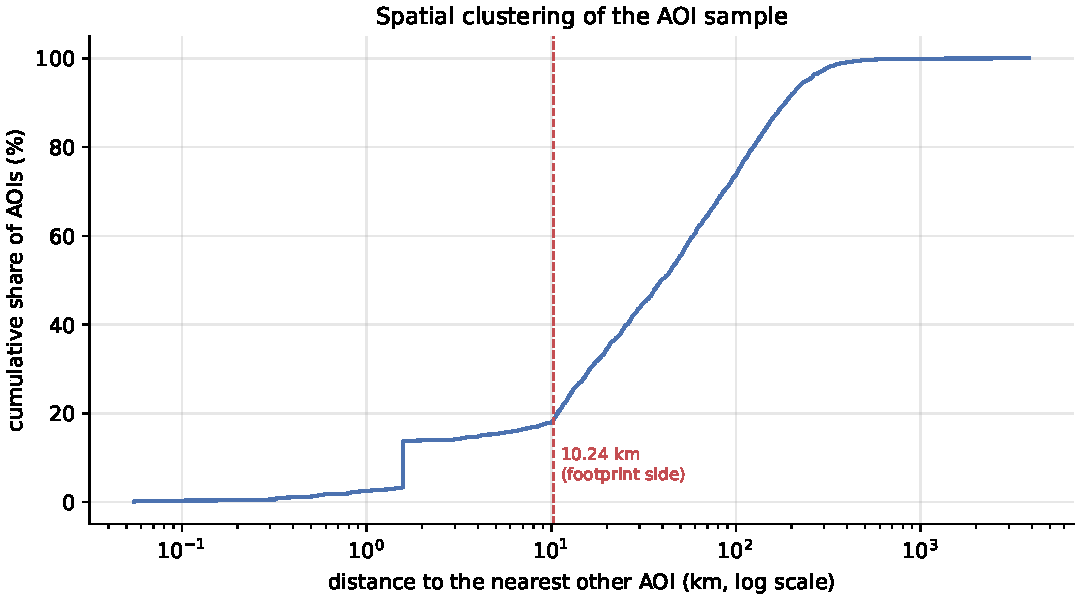
\includegraphics[width=0.78\textwidth]{clustering.pdf}
\caption{Cumulative distribution of the distance to the nearest other AOI. The dashed line is
the footprint width: everything to its left produces overlapping imagery.}
\label{fig:clustering}
\end{figure}

With our enlarged footprint this produces \OverlapPairs{} overlapping pairs involving
\OverlapSites{} AOIs. \CrossSplitPairs{} of those pairs join AOIs that WorldStrat assigns to
\emph{different} splits (1\,291 train/test, 1\,057 train/validation). Inheriting the WorldStrat
splits would therefore leak pixels between training and evaluation --- not a flaw of WorldStrat,
whose $2.5\,\mathrm{km}^2$ tiles do not overlap, but a direct consequence of sampling
$104.9\,\mathrm{km}^2$ around each centre. Grouping AOIs into spatial blocks (a $0.5^\circ$
grid yields 2\,771 groups) and splitting by block removes it.

\subsection{A bias the list cannot fix: clear-sky selection}

One more effect deserves mention because it appears at download time rather than in the list.
Selecting scenes by cloud cover (\texttt{--max\_cloud}) biases the sample towards the dry season,
and the strength of that bias depends on climate: an arid site will return usable scenes all
year, while a tropical site may only pass the threshold for a few months. Two mitigations are
available in the pipeline: widen the date range per site, or raise \texttt{--max\_cloud} and use
the per-scene cloud statistics already recorded in \texttt{metadata.csv} to filter afterwards.

\section{Recommendations}

\begin{enumerate}
  \item \textbf{Use the list as-is for pre-training and super-resolution.} Scene diversity, not
        equal-area coverage, is what matters there, and the humanitarian sources are an asset.
  \item \textbf{Do not use it for global statistics} (area estimation, land-cover priors,
        climate-wide generalisation claims) without reweighting by $1/r_c$ or subsampling to
        match land area. The rarest strata cap what subsampling can achieve: with 121 polar and
        103 Oceanian AOIs, a land-proportional subsample is limited to roughly 800 sites.
  \item \textbf{Split spatially, not by AOI.} Use $0.5^\circ$ blocks (or any grouping wider than
        the footprint) rather than the inherited WorldStrat splits.
  \item \textbf{Consider a complementary equal-area list.} \texttt{run\_sites.py} accepts any
        CSV, so a few hundred points drawn uniformly over the Köppen land mask --- weighted
        towards the deficient strata (B, D, E, Oceania) --- would be enough to rebalance the
        dataset. This is a small addition to \texttt{build\_worldstrat\_aoi.py} and can be
        produced on request.
  \item \textbf{Record the biases with the dataset.} The annotated CSV
        (\texttt{report/generated/aoi\_annotated.csv}) carries the climate, continent and
        land-cover label of every AOI, which is what downstream users need to reweight.
\end{enumerate}

\section{Cost of a full run}

One acquisition occupies 19.1\,MB on disk (13 bands, validity and quality masks, compressed),
measured on a real output. Storage therefore scales as
$\NAOI \times n_\text{dates} \times 19.1\,\mathrm{MB}$:

\begin{center}
\begin{tabular}{lrr}
\toprule
Scenario & Dates per site & Total volume \\
\midrule
One clear scene per site           & 1  & 75\,GB \\
Seasonal (one per quarter, 1 year) & 4  & 300\,GB \\
Monthly, 1 year                    & 12 & 900\,GB \\
Monthly, 2 years                   & 24 & 1.8\,TB \\
\bottomrule
\end{tabular}
\end{center}

Two practical constraints follow from the test runs. The CDSE catalogue rate-limits bursts of
queries (HTTP 429), which is why \texttt{run\_sites.py} pauses between sites and retries with
exponential back-off; and S3 access is markedly faster than the HTTPS fallback, which
transfers whole band files. For a first full build we suggest a pilot of a few hundred sites
sharded with \texttt{--skip}/\texttt{--limit}, which also gives a reliable throughput estimate
before committing to terabytes.

\section{Conclusion}

The coordinate list is ready and scripted end to end. Its biases are now measured rather than
assumed: a two-order-of-magnitude built-up over-representation, a \ratio{1.9}/\ratio{0.2}
temperate-to-polar imbalance, thin coverage of Oceania and of the world's deserts, and enough
spatial clustering to require spatial splitting. All of them are recorded per AOI in the
annotated CSV, so they can be corrected by reweighting or by a complementary equal-area sample
rather than by discarding the list.

\appendix
\section{Köppen--Geiger classes}
\label{app:classes}

\begin{table}[H]
\centering
\caption{The 15 most frequent Köppen--Geiger classes among the AOIs.}
\begin{tabular}{lrrrr}
\toprule
K\"oppen class & AOIs & sample (\%) & land (\%) & ratio \\
\midrule
Aw & 573 & 14.6 & 11.4 & 1.28 \\
Af & 454 & 11.6 & 5.0 & 2.30 \\
BSh & 362 & 9.2 & 5.3 & 1.74 \\
BWh & 358 & 9.1 & 14.7 & 0.62 \\
Cfa & 304 & 7.7 & 3.8 & 2.06 \\
Dfb & 285 & 7.3 & 5.0 & 1.45 \\
BSk & 186 & 4.7 & 6.0 & 0.79 \\
Csa & 169 & 4.3 & 1.0 & 4.24 \\
Am & 164 & 4.2 & 3.5 & 1.19 \\
Cfb & 159 & 4.1 & 1.8 & 2.26 \\
Dfa & 147 & 3.7 & 1.3 & 2.78 \\
Cwa & 143 & 3.6 & 2.8 & 1.30 \\
Dfc & 141 & 3.6 & 10.5 & 0.34 \\
Dwa & 117 & 3.0 & 0.8 & 3.64 \\
BWk & 89 & 2.3 & 5.1 & 0.44 \\
\bottomrule
\end{tabular}

\end{table}

\begin{figure}[H]
\centering
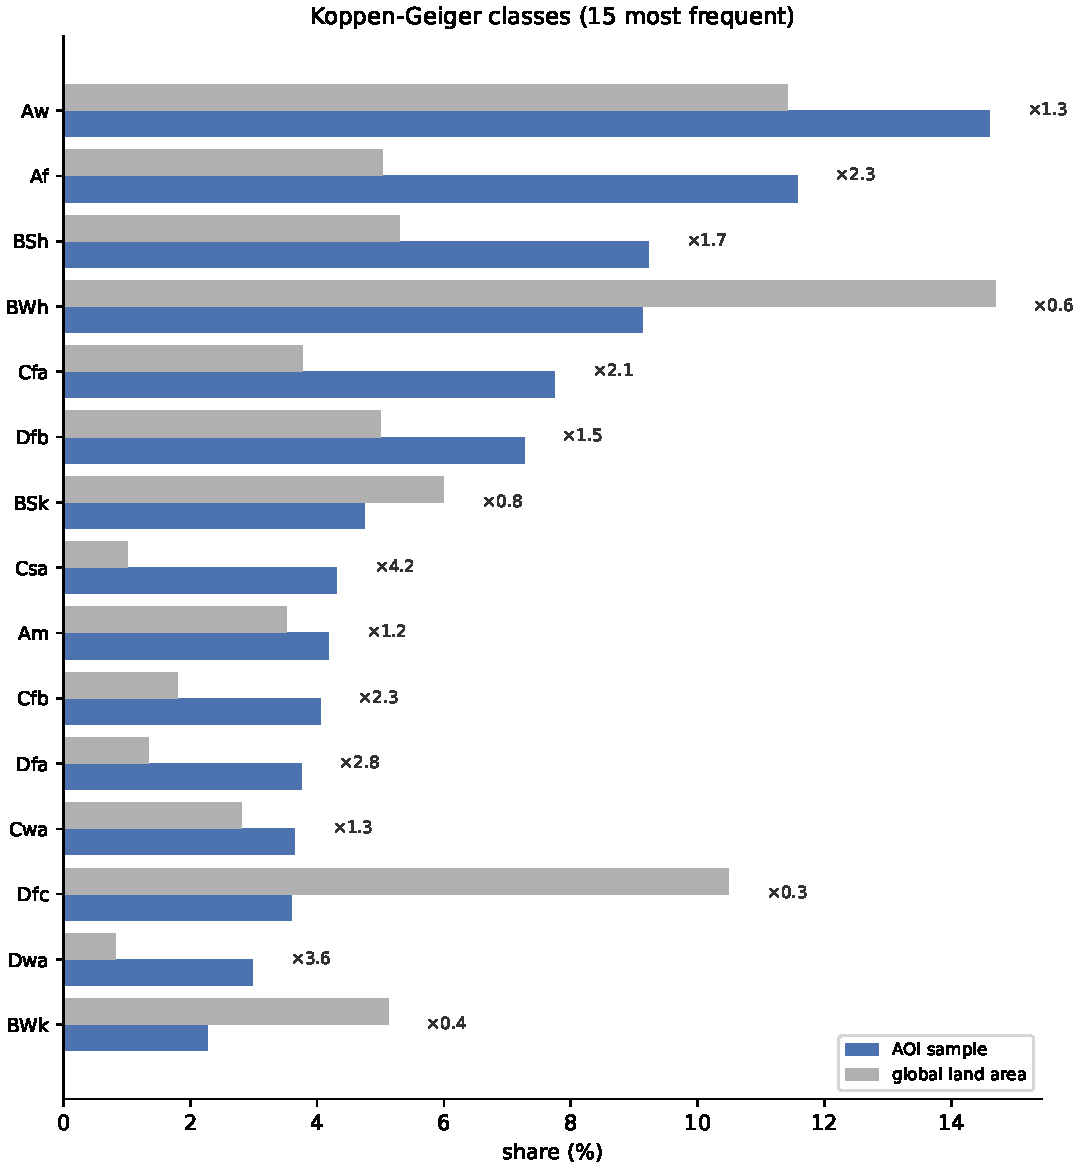
\includegraphics[width=0.85\textwidth]{koppen_classes.pdf}
\caption{Köppen--Geiger classes: sample versus global land area.}
\end{figure}

\section{Reproduction and data licences}

\begin{verbatim}
pip install -r requirements.txt          # pipeline
pip install pandas scipy matplotlib      # analysis only
python build_worldstrat_aoi.py           # -> sites/worldstrat_aoi.csv
python analyze_aoi_bias.py               # -> report/figures, report/generated
pdflatex worldstrat_aoi_report.tex       # -> this PDF
\end{verbatim}

WorldStrat metadata: CC-BY-4.0 \cite{worldstrat}. Köppen--Geiger map: CC-BY-4.0 \cite{koppen}.
Natural Earth: public domain. Sentinel-2 imagery: Copernicus open licence, accessed through the
Copernicus Data Space Ecosystem.

\begin{thebibliography}{9}
\bibitem{worldstrat}
J.~Cornebise, I.~Oršolić, F.~Kalaitzis,
\emph{Open High-Resolution Satellite Imagery: The WorldStrat Dataset --- With Application to
Super-Resolution},
NeurIPS Datasets and Benchmarks, 2022. Zenodo record 6810792.

\bibitem{koppen}
H.~E.~Beck, N.~E.~Zimmermann, T.~R.~McVicar, N.~Vergopolan, A.~Berg, E.~F.~Wood,
\emph{Present and future Köppen--Geiger climate classification maps at 1-km resolution},
Scientific Data 5:180214, 2018.

\bibitem{ghsl}
M.~Pesaresi et al.,
\emph{Global Human Settlement Layer (GHSL): built-up surface},
European Commission, Joint Research Centre. Built-up surface is of the order of 1\% of the
ice-free land surface.
\end{thebibliography}

\end{document}
